\documentclass{book}

\usepackage[a4paper]{geometry}

\usepackage[T2A]{fontenc}
\usepackage[utf8]{inputenc}
\usepackage[english,russian]{babel}

\usepackage{graphicx}

\begin{document}

\tableofcontents

\part{Описание конструктора}

\chapter{Релейная логика}

\part{Лабораторные работы}

\chapter{Калькулятор}

\section{Тумблеры}

Модуль с тумблерами используется для ручного включения и выключения реле.
Присоединяя его к разным разъёмам, можно задавать четырёхбитное число,
либо переключать до четырёх управляющих сигналов.

Проще всего проверить работу тумблеров, подключив их к управляющей шине
регистрового модуля, в который вставлены только $4$ реле.

\subsection{Практикум}

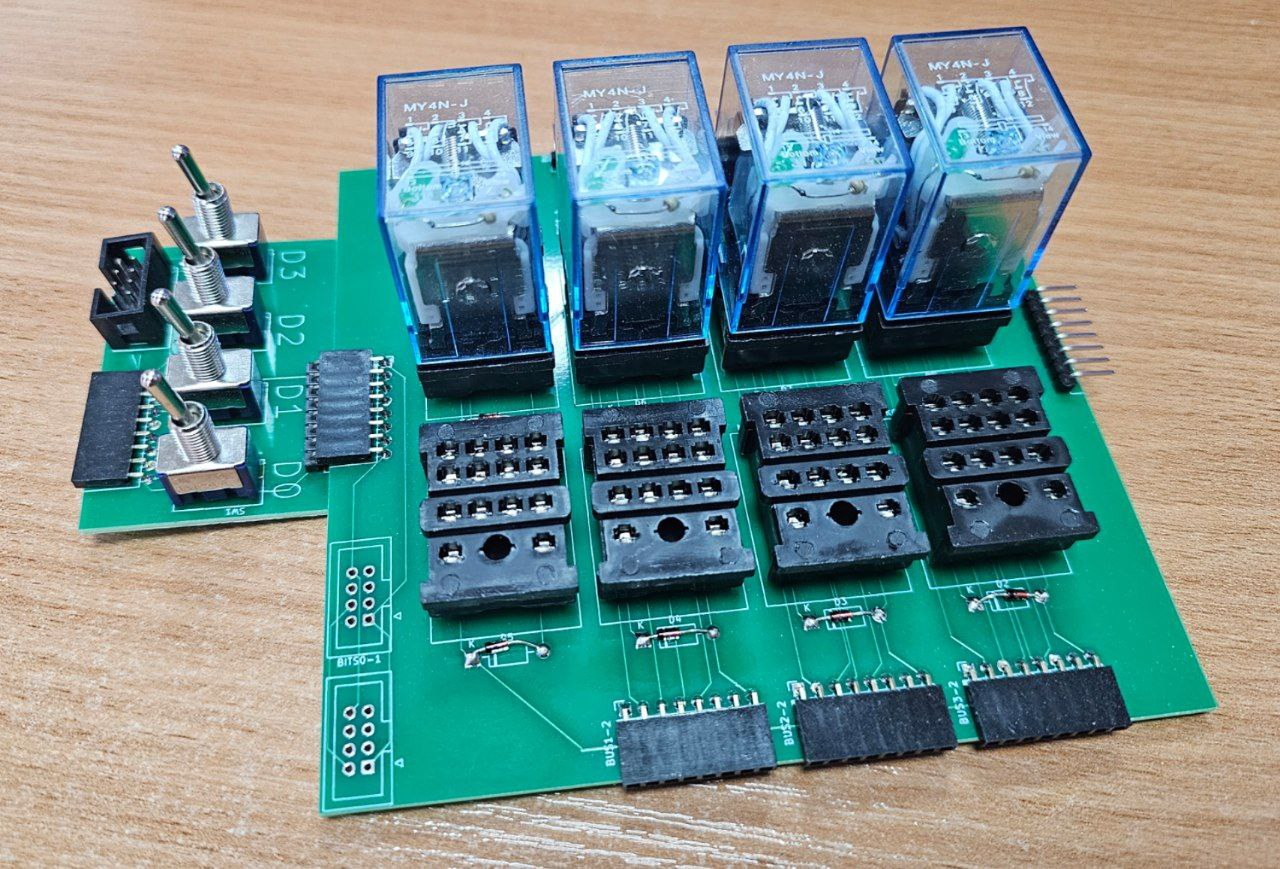
\includegraphics[width=\columnwidth]{photo/switches.jpg}

\begin{enumerate}
    \item Переключать тумблеры. Убедиться, что положение одного тумблера меняет состояние одного реле.
    \item Запомнить включенное и выключенное состояния тумблера, чтобы позднее не было проблем с управлением другими схемами.
\end{enumerate}

\section{Регистр}

Модуль четырёхбитного регистра состоит из четырёх реле-триггеров,
одного реле для обнуления регистра и трёх реле для подключения
к шинам данных.

Модуль <<Регистр>> имеет следующие разъёмы:
\begin{itemize}
  \item Слева и справа: управляющие сигналы сброса и выборки.
        Можно подключить тумблеры
        для ручного включения сигналов. Также можно соединить несколько
        модулей регистра, чтобы управлять одним набором сигналов сразу
        для $8$, $12$ \ldots бит.
  \item Сверху и снизу: три шины данных. Реле регистра могут
        подключаться к шинам для записи или чтения данных.
  \item Дополнительные разъёмы с битами $0-3$ и $2-3$ для чтения или
        записи значения без подключения к шине.
\end{itemize}

\subsection{Практикум}

Протестировать работу регистра можно собрав следующую схему:

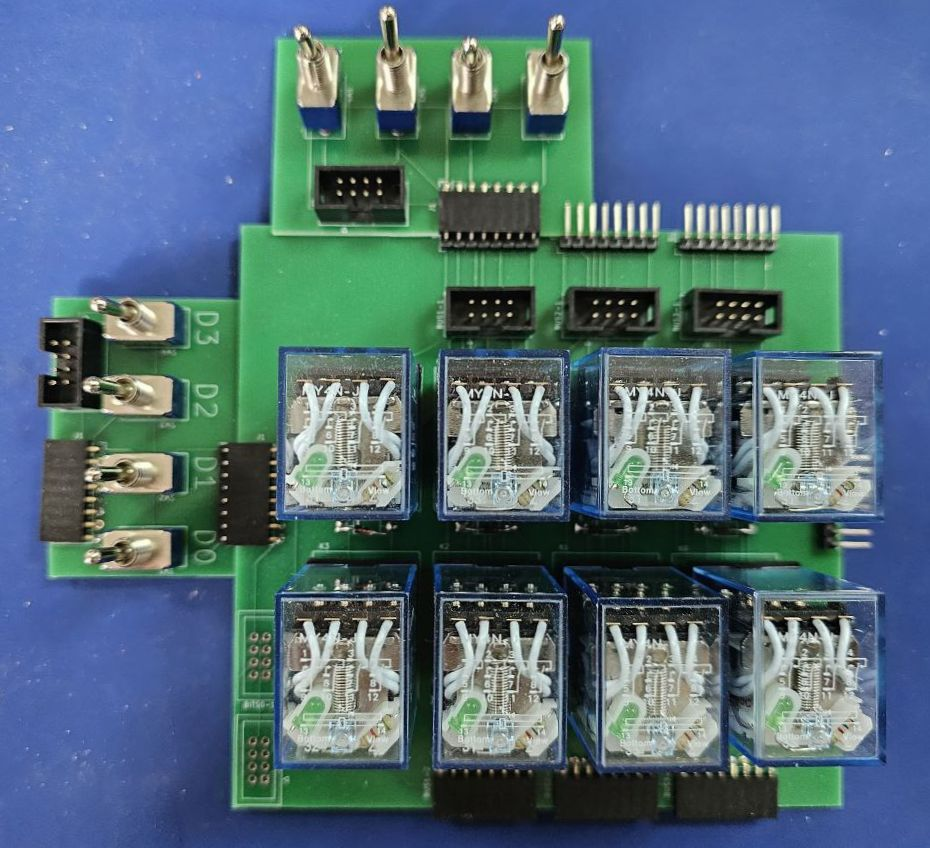
\includegraphics[width=\columnwidth]{photo/register.jpg}

\begin{itemize}
  \item Тумблеры слева управляют работой регистра. Бит 0 --- обнуление, бит 1 --- выборка на шину 1.
  \item Тумблеры сверху нужны для ввода значения регистра. Когда он подключается к шине 1,
        значения, набранное на тумблерах, записывается в регистр.
\end{itemize}

\subsubsection{Регистр без шины}

\begin{enumerate}
    \item Подключить тубмлеры проводом к битам $0-3$ вместо шины.
    \item Набирать значение, убедиться, что биты переключаются в $1$, но не возвращаются в $0$.
    \item Обнулить тумблеры с данными.
    \item Включить и выключить сигнал сброса. Убедиться, что значения всех битов теперь $0$.
\end{enumerate}

\subsubsection{Регистр с шиной}

\begin{enumerate}
    \item Отключить все управляющие сигналы.
    \item Набрать значение на тумблерах для данных. Убедиться, что это не влияет на регистр.
    \item Включить и выключить сигнал выборки на шину $1$. Убедиться, что данные записались в регистр.
    \item Включить и выключить сигнал сброса. Убедиться, что значения всех битов теперь $0$.
\end{enumerate}

\section{Шина и регистровый файл}

\section{Унарные логические операции}

\section{Сложение}

\section{Бинарные логические операции}

\section{Вычитание}

\section{Целый калькулятор}

\chapter{Элементы компьютера}

\chapter{Компьютер}

\end{document}
